%% LyX 2.0.3 created this file.  For more info, see http://www.lyx.org/.
%% Do not edit unless you really know what you are doing.
\documentclass[english]{article}
\usepackage[T1]{fontenc}
\usepackage[latin9]{inputenc}
\usepackage{float}
\usepackage{graphicx}
\usepackage{babel}
\begin{document}

\title{Susceptibility computation for Ising model for 2D and 1D}

\maketitle
This is short theoretical explanation of the test: \textbf{IsingTestChi1D.h}
and \textbf{IsingTestChi2D.h}.


\section{Theory}

Magnetic susceptibility ($\chi$) is defined by the relationship:
\[
\chi=\frac{\partial M}{\partial h},
\]


where $M$ is magnetization of the system
\[
M=\sum_{i}s_{i}
\]


and $h$ is magnetic field strength. We focus on calculating the magnetic
susceptibility at zero magnetic field:

\[
\chi_{0}=\frac{\partial M}{\partial h}|_{h=0},
\]


calculated per one site.

For the system of spins $s_{i}$ in external magnetic field $h$,
the Hamiltonian is:

\[
\hat{H}=J\sum_{\left\langle i,j\right\rangle }s_{i}s_{j}+h\sum_{i}s_{i},
\]


where $\beta=1/(k_{B}T)$, $J$ is interaction energy between the
adjacent spins and the first sum runs over pairs of neighboring sites
$s_{i}$.

We can calculate $\chi_{0}$ as:

\[
\chi_{0}=\frac{\partial\left\langle M\right\rangle }{\partial h}.
\]


Here the value of magnetization is averaged over the configurations
$\{s\}$ of spins:

\begin{equation}
\left\langle M\right\rangle =\frac{1}{Z}\sum_{\{s\}}M\exp(-\beta J\sum_{\left\langle i,j\right\rangle }s_{i}s_{j}-\beta h\sum_{i}s_{i}),\label{eq:meanM}
\end{equation}


where 
\[
Z=\sum_{\{s\}}\exp(-\beta J\sum_{\left\langle i,j\right\rangle }s_{i}s_{j}-\beta h\sum_{i}s_{i}).
\]


To obtain a formula useful for the numerical calculation of $\chi_{0}$,
let us take the derivative of the (\ref{eq:meanM}) with respect to
$h$. 

\[
\frac{\partial\left\langle M\right\rangle }{\partial h}=\frac{\beta}{Z}\sum_{\{s\}}M^{2}\exp(-\beta\hat{H})-\frac{\beta}{Z^{2}}\left[\sum_{\{s\}}M\exp(-\beta\hat{H})\right]^{2}=\beta\left(\left\langle M^{2}\right\rangle -\left\langle M\right\rangle ^{2}\right).
\]


In zero field:

\[
\chi_{0}=\beta\left(\left\langle M^{2}\right\rangle |_{h=0}-\left\langle M\right\rangle ^{2}|_{h=0}\right).
\]


This formula allows for calculation of the $\chi_{0}$ in the Monte
Carlo simulation of Ising model. 

For comparison of the numerical results with the theoretical values
of the magnetization, let us consider the behavior of $\chi_{0}$
in function of the temperature. In one dimension, for a chain of $N$spins
the analytical formula is:

\begin{equation}
\chi_{0}=\frac{\beta}{N}\exp\left(2\beta J\right).\label{eq:1Dchi_an}
\end{equation}


For 2D square lattice of $N$ spins we don't have the exact formula
for the susceptibility, but we know the behavior in the critical temperature:

\[
\chi\sim\left|t\right|^{-\gamma},
\]


where $t=\frac{T-T_{c}}{T_{c}}$, $T_{c}$ being the critical temperature,
and $\gamma$ is the critical exponent. For an infinite 2D lattice
their values are:

\[
T_{c}=2.269,\:\gamma=7/4.
\]
It means that for the critical temperature the magnetic susceptibility
diverges at $t$. For finite lattice the critical temperature is slightly
different. The susceptibility 


\section{Results for 1D chain}

The appropriate test class has name: IsingTestChi1D.

We performed the calculations of $\chi_{0}$versus the temperature
for a chain of $N=500$ spins. We compared the results with the analytical
solution. The dependence is shown in the figure (\ref{chi_T}). For
high temperatures we find a good agreement with the analytical solution.
However, for low temperatures there is a significant difference between
the numerical and analytical results. We attribute this behavior to
the low acceptance ratio of Metropolis algorithm, which lowers the
number of configurations used in the averaging. 

\begin{figure}[H]
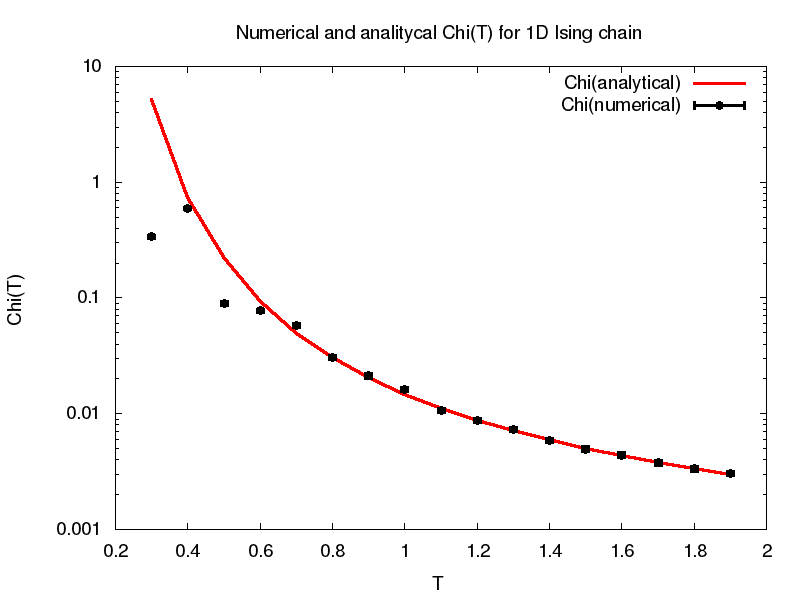
\includegraphics[width=0.6\paperwidth]{IsingTestChi1D}\label{chi_T}

\caption{The numerical and analytical results for susceptibility versus the
temperature. The plot is generated by the IsingTestChi1D class.}
\end{figure}


Also, we performed the calculations of the magnetic susceptibility
versus the number of spins at $T=1$ K. According to (\ref{eq:1Dchi_an}),
$\chi_{0}$ is proportional to inverse $N$. Results are shown on
Fig. \ref{chi_N}. We find a good agreement with the analytical solution.

\begin{figure}[H]
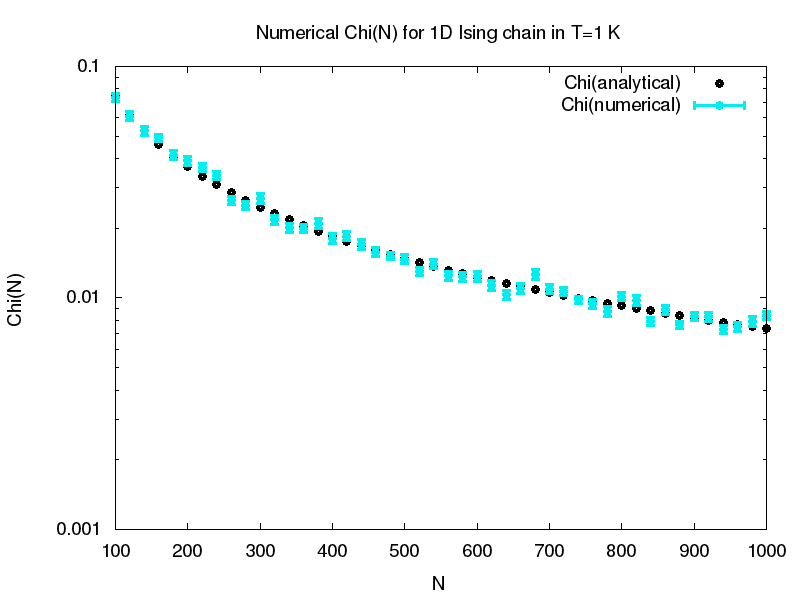
\includegraphics[width=0.6\paperwidth]{IsingTestChi1D_N}\label{chi_N}

\caption{The numerical and analytical results for susceptibility versus the
size of chain. }


\end{figure}



\section{Results for 2D lattice}

The appropriate test class has name: IsingTestChi2D. 

We computed the susceptibility versus temperature for a square lattice
consisting of 90000 spins. The results are shown in figure \ref{chi_E2D}.
For each $T$ we did 100000 iterations. We plot also a function showing
the critical behavior for infinite lattice for comparison, from the
right side of the critical point, using arbitrary proportionality
factor $7\cdot10^{-6}$.

\begin{figure}[H]
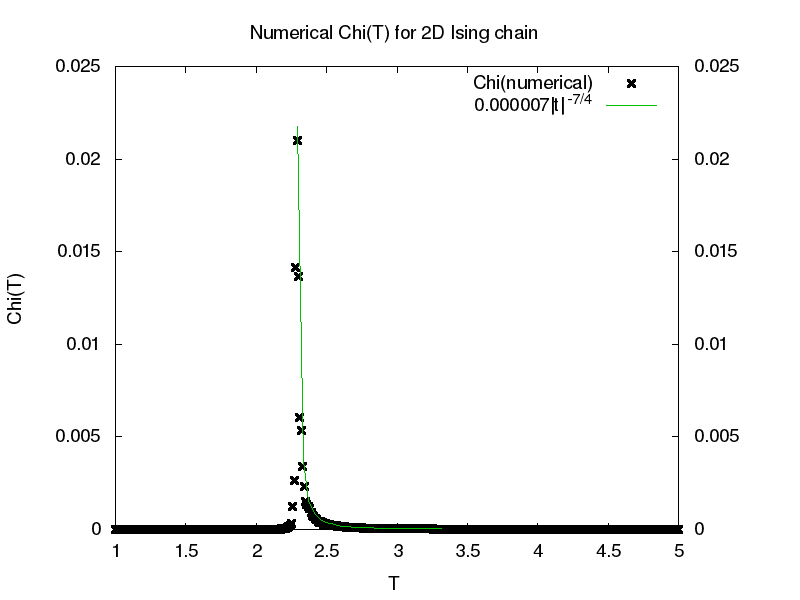
\includegraphics[width=0.6\paperwidth]{IsingTestChi2D}\label{chi_E2D}

\caption{Results for susceptibility versus the temperature. Green line shows
the critical behavior for infinite lattice from the right side of
the critical point.}


\end{figure}


The test IsingTestChi2D performs the calculations for a lattice $20\times20$
spins.
\end{document}
